

Leptoquarks can be scalar (spin 0) or vector (spin 1) bosons, are color-triplets under \SUthreeC, carry fractional electric charge and weak isospin. Listed in Table~\ref{tab:LQModels} are the possible quantum numbers a leptoquark may take assuming dimensionless couplings to SM fermions and invariance under the gauge group of the SM. The first two columns list the spin and fermion quantum numbers, followed by the QCD and weak isospin representations, the weak hypercharge, and the allowed couplings to chiral SM fermions (color indices, flavor indices, and charge conjugates have been supressed). As the right-most column of Table~\ref{tab:LQModels} shows, leptoquarks may couple to only right-chiral fermions or left-chiral fermions, called chiral leptoquarks, or one left-chiral and one right-chiral fermion, called non-chiral leptoquarks. The allowed lepton and quark generations have historically been constrained to the same generation, motived by experimental limits placed on rare processes like proton decay, and FCNCs~\cite{FCNC}. However, as detailed in Section~\ref{sec:ExperimentalMotivation}, allowing intergenerational mixing can provide an explaination for phenomena like the flavor anomalies and muon magnetic moment anomaly. 

For a given leptoquark model there are also a set of free parameters, which include the mass \MLQ the Yukawa coupling at the leptoquark-quark-lepton vertex $\lambda$, and the decay branching fraction into a charged lepton $\beta$ (with $\beta-1$ the branching fraction into a neutrino). Specific to vector leptoquark models are two additional parameters $\lambda_{\text{G}}$ and $\kappa_{\text{G}}$ that correspond to the couplings of leptoquarks to SM gauge bosons at the \HepProcess{\Pgluon\LQ} and \HepProcess{\Pgluon\Pgluon\LQ} vertices. The LHC is capable of both single- and pair-production of leptoquarks through large QCD cross sections, as shown in Figs.~\ref{fig:LQsingleprod} and~\ref{fig:LQpairprod}. 

\begin{table}[H]
    \begin{center}
        \caption{List of quantum numbers and allowed couplings to quarks/leptons for different leptoquark models.}
        \begin{tabular}{cccccl}
            \hline \hline
            Spin    & $3B+L$    & \SUthreeC                                 & \SUtwoW   & \UoneY        & Allowed coupling \\ \hline
            \num{0} & \num{-2}  & \num[parse-numbers=false]{\overline{3}}   & \num{1}   & \num{1/3}     & $\antispinor{\Pquark}{L}{c}\spinor{\Plepton}{L}{}$ or $\antispinor{\Pup}{R}{c}\spinor{\Pe}{R}{}$ \\ 
            \num{0} & \num{-2}  & \num[parse-numbers=false]{\overline{3}}   & \num{1}   & \num{4/3}     & $\antispinor{\Pdown}{R}{c}\spinor{\Pe}{R}{}$ \\ 
            \num{0} & \num{-2}  & \num[parse-numbers=false]{\overline{3}}   & \num{3}   & \num{1/3}     & $\antispinor{\Pquark}{L}{c}\spinor{\Plepton}{L}{}$ \\ 
            \num{1} & \num{-2}  & \num[parse-numbers=false]{\overline{3}}   & \num{2}   & \num{5/6}     & $\antispinor{\Pquark}{L}{c}\gammamu\spinor{\Pe}{R}{}$ or $\antispinor{\Pdown}{R}{c}\gammamu\spinor{\Plepton}{L}{}$ \\ 
            \num{1} & \num{-2}  & \num[parse-numbers=false]{\overline{3}}   & \num{2}   & \num{-1/6}    & $\antispinor{\Pup}{R}{c}\gammamu\spinor{\Plepton}{L}{}$ \\ 
            \num{0} & \num{0}   & \num{3}                                   & \num{2}   & \num{7/6}     & $\antispinor{\Pquark}{L}{}\spinor{\Pe}{R}{}$ or $\antispinor{\Pup}{R}{}\spinor{\Plepton}{L}{}$ \\ 
            \num{0} & \num{0}   & \num{3}                                   & \num{2}   & \num{1/6}     & $\antispinor{\Pdown}{R}{}\spinor{\Plepton}{L}{}$ \\ 
            \num{1} & \num{0}   & \num{3}                                   & \num{1}   & \num{2/3}     & $\antispinor{\Pquark}{L}{}\gammamu\spinor{\Plepton}{L}{}$ or $\antispinor{\Pdown}{R}{}\gammamu\spinor{\Pe}{R}{}$ \\ 
            \num{1} & \num{0}   & \num{3}                                   & \num{1}   & \num{5/3}     & $\antispinor{\Pup}{R}{}\gammamu\spinor{\Pe}{R}{}$ \\ 
            \num{1} & \num{0}   & \num{3}                                   & \num{3}   & \num{2/3}     & $\antispinor{\Pquark}{L}{}\gammamu\spinor{\Plepton}{L}{}$ \\ \hline \hline
        \end{tabular}
        \label{tab:LQModels}
    \end{center}
\end{table}

\begin{figure}[H]
    \centering
    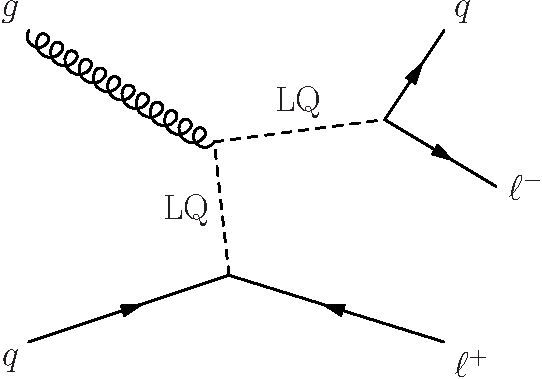
\includegraphics[width=0.3\textwidth]{Images/Theory/SingleLQProdT1.pdf}\hspace{0.1\textwidth}
    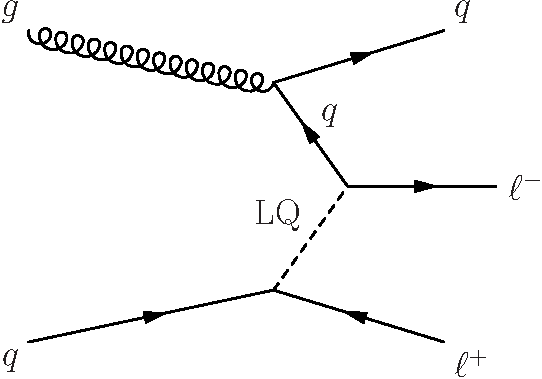
\includegraphics[width=0.3\textwidth]{Images/Theory/SingleLQProdT2.pdf}\vspace{0.05\textwidth}
    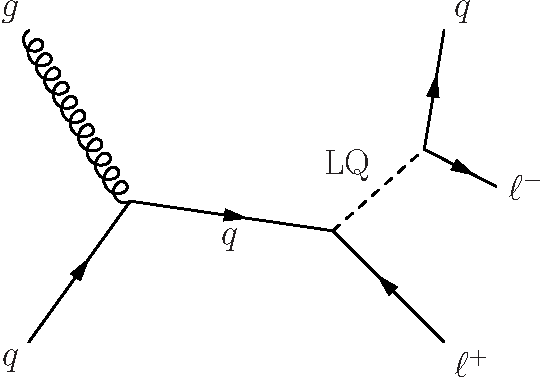
\includegraphics[width=0.3\textwidth]{Images/Theory/SingleLQProdS1.pdf}\vspace{0.05\textwidth}
    \caption{Production mechanisms of single leptoquarks at the LHC. Clockwise from top left: a t-channel processes that results in a resonant \HepProcess{\Pquark\Plepton} pair and a non-resonant \Plepton, a t-channel processes resulting in a non-resonant \HepProcess{\Plepton\Plepton\Pquark} final state, and an t-channel process resulting in a resonant \HepProcess{\Pquark\Plepton} pair and a non-resonant \Plepton.}
    \label{fig:LQsingleprod}
\end{figure}

\begin{figure}[H]
    \centering
    \includegraphics[width=0.3\textwidth]{Images/Theory/LQLQProduction_1.pdf}\hspace{0.1\textwidth}
    \includegraphics[width=0.3\textwidth]{Images/Theory/LQLQProduction_3.pdf}\vspace{0.05\textwidth}
    \includegraphics[width=0.3\textwidth]{Images/Theory/LQLQProduction_2.pdf}\hspace{0.1\textwidth}
    \includegraphics[width=0.3\textwidth]{Images/Theory/LQLQProduction_4.pdf}\vspace{0.05\textwidth}
    \caption{Production mechanisms of \HepProcess{\LQ\LQbar} pairs at the LHC. Clockwise from top-left: s-channel gluon-gluon fusion, gluon-gluon four-point interaction, t-channel gluon-gluon interaction via leptoquark exchange, and s-channel quark-antiquark annihilation.}
    \label{fig:LQpairprod}
\end{figure}